\section{graphs and other tikz}
 \frame{\sectionpage}
 
\begin{frame}{Drawning within tikz}
    \tikzset{every picture/.style={line width=0.75pt}} %set default line width to 0.75pt        

\begin{tikzpicture}[x=0.75pt,y=0.75pt,yscale=-1,xscale=1]
%uncomment if require: \path (0,486); %set diagram left start at 0, and has height of 486

%Curve Lines [id:da9595099437611456] 
\draw    (233.23,183.24) .. controls (252.87,215.34) and (288.86,227.45) .. (323.09,223.22) .. controls (353.65,219.45) and (382.81,202.65) .. (397.65,175.44) ;
%Curve Lines [id:da6932103982097759] 
\draw    (244.67,197.26) .. controls (301.86,150.51) and (339.03,156.74) .. (383.35,191.03) ;
%Curve Lines [id:da7053828945347995] 
\draw    (126,173.88) .. controls (131.72,222.2) and (184.62,311.04) .. (317.59,307.92) .. controls (450.55,304.8) and (507.74,212.85) .. (499.16,173.88) ;
%Curve Lines [id:da583602680611125] 
\draw    (126,173.88) .. controls (174.61,52.32) and (437.68,50.76) .. (499.16,173.88) ;
%Curve Lines [id:da5190289437371578] 
\draw [color={rgb, 255:red, 208; green, 2; blue, 27 }  ,draw opacity=1 ]   (126,173.88) .. controls (175,318) and (478,278) .. (499.16,173.88) ;
%Curve Lines [id:da5494113181101443] 
\draw [color={rgb, 255:red, 74; green, 144; blue, 226 }  ,draw opacity=1 ]   (313,222) .. controls (294,238) and (299,291) .. (317.59,307.92) ;
%Curve Lines [id:da8828117501564781] 
\draw [color={rgb, 255:red, 74; green, 144; blue, 226 }  ,draw opacity=1 ] [dash pattern={on 0.84pt off 2.51pt}]  (313,222) .. controls (330,233) and (336,298) .. (317.59,307.92) ;
%Shape: Parallelogram [id:dp02778297397005436] 
\draw  [fill={rgb, 255:red, 144; green, 144; blue, 144 }  ,fill opacity=0.44 ] (145.57,94) -- (308.5,94) -- (238.68,242.38) -- (75.75,242.38) -- cycle ;
%Shape: Circle [id:dp8371213746664339] 
\draw  [color={rgb, 255:red, 253; green, 1; blue, 1 }  ,draw opacity=1 ][fill={rgb, 255:red, 255; green, 0; blue, 0 }  ,fill opacity=1 ] (195.13,164.19) .. controls (195.13,163.08) and (196.02,162.19) .. (197.13,162.19) .. controls (198.23,162.19) and (199.13,163.08) .. (199.13,164.19) .. controls (199.13,165.29) and (198.23,166.19) .. (197.13,166.19) .. controls (196.02,166.19) and (195.13,165.29) .. (195.13,164.19) -- cycle ;
%Straight Lines [id:da21346648436809335] 
\draw [color={rgb, 255:red, 65; green, 117; blue, 5 }  ,draw opacity=1 ]   (197.13,164.19) -- (181.9,194.22) ;
\draw [shift={(181,196)}, rotate = 296.88] [color={rgb, 255:red, 65; green, 117; blue, 5 }  ,draw opacity=1 ][line width=0.75]    (10.93,-3.29) .. controls (6.95,-1.4) and (3.31,-0.3) .. (0,0) .. controls (3.31,0.3) and (6.95,1.4) .. (10.93,3.29)   ;

% Text Node
\draw (501,122.4) node [anchor=north west][inner sep=0.75pt]    {$\ $};
% Text Node
\draw (478,109) node [anchor=north west][inner sep=0.75pt]   [align=left] {\(\mathbb{T}\)};
% Text Node
\draw (82,65) node [anchor=north west][inner sep=0.75pt]   [align=left] {\(T_x\mathbb{T}\)};
% Text Node
\draw (206,152) node [anchor=north west][inner sep=0.75pt]   [align=left] {\textcolor{red2}{{\footnotesize \(x\)}}};
% Text Node
\draw (191.06,183.09) node [anchor=north west][inner sep=0.75pt]   [align=left] {{\footnotesize \textcolor{green2}{\(v\)}}};

\end{tikzpicture}

    
\end{frame}



\begin{frame}{It's possible plotting graphs with pgfplots and tikz}

\centering
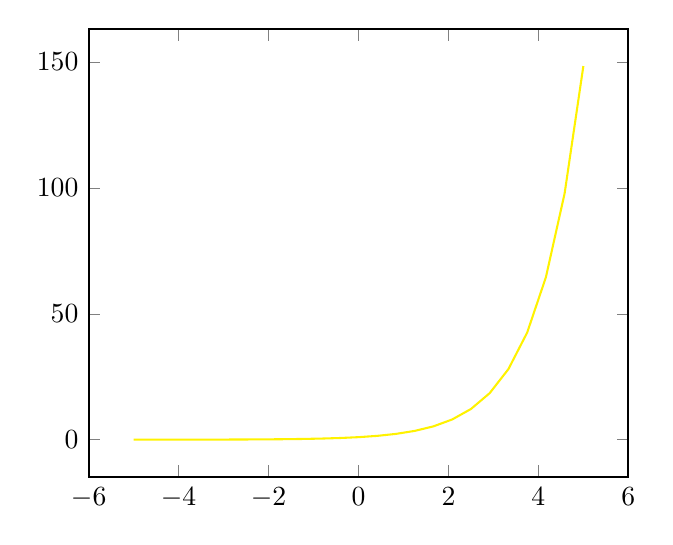
\begin{tikzpicture}
\begin{axis}
\addplot[color=yellow]{exp(x)};
\end{axis}
\end{tikzpicture}
%Here ends the 2D plot

%Here ends the 3D plot

\end{frame}

\begin{frame}{Plotting 3d}
%Here begins the 3D plot
\centering
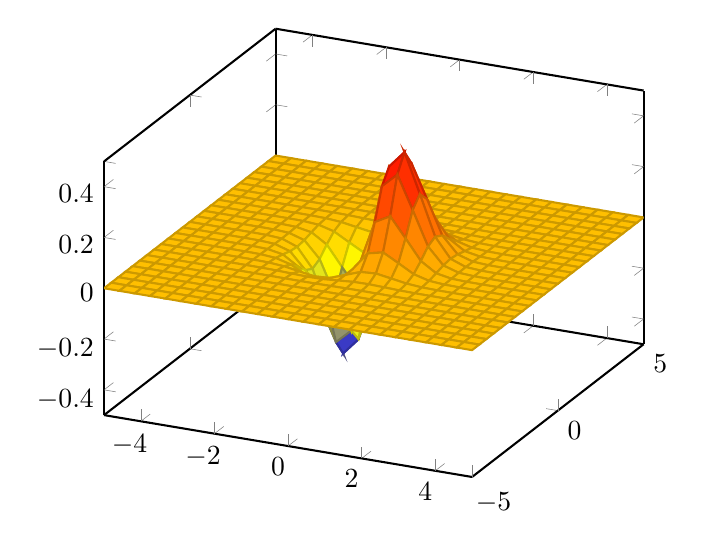
\begin{tikzpicture}
\begin{axis}
\addplot3[
    surf,
]
{exp(-x^2-y^2)*x};
\end{axis}
\end{tikzpicture}
\end{frame}
